\documentclass[crop, tikz]{standalone}
\usepackage{tikz}

\usetikzlibrary{arrows,shapes, decorations.pathmorphing,backgrounds,positioning}
\usetikzlibrary{decorations.pathreplacing}
\usetikzlibrary{arrows.meta}

\tikzstyle{smallnode}=[draw, circle, inner sep=2pt]
\tikzstyle{invis}=[inner sep=2pt]
\tikzstyle{stateTransition}=[thick, ->, -{Latex[length=3mm,width=3mm]}, align=center]


\begin{document}
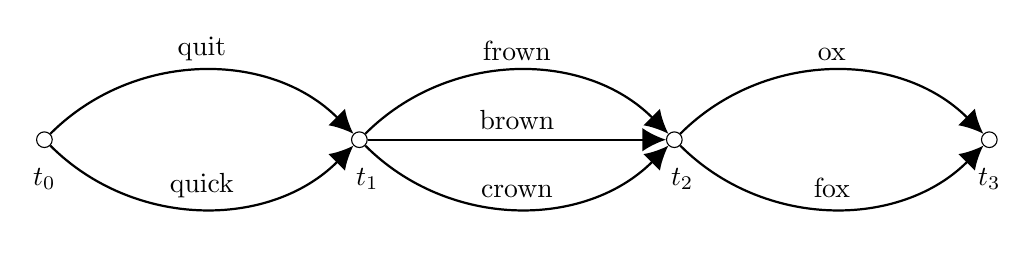
\begin{tikzpicture}
    % nodes
    \node[smallnode] (n1) at (-4, 0) {};
    \node[invis] (t1) at (-4, -0.5) {$t_0$};
    \node[smallnode] (n2) at (0, 0) {};
    \node[invis] (t2) at (0.1, -0.5) {$t_1$};
    \node[smallnode] (n3) at (4, 0) {};
    \node[invis] (t3) at (4.1, -0.5) {$t_2$};
    \node[smallnode] (n4) at (8, 0) {};
    \node[invis] (t4) at (8, -0.5) {$t_3$};

    % 1-Best Arcs
	\draw[stateTransition] (n1) to[out=-45,in=-135] node [midway, sloped, above] {quick} (n2);
	\draw[stateTransition] (n2) to[out=0,in=180] node [midway, sloped, above] {brown} (n3);
	\draw[stateTransition] (n3) to[out=-45,in=-135] node [midway, sloped, above] {fox} (n4);
	
	% Confusion Network Arcs
	\draw[stateTransition] (n1) to[out=45,in=135] node [midway, sloped, above] {quit} (n2);
	\draw[stateTransition] (n2) to[out=45,in=135] node [midway, sloped, above] {frown} (n3);
	\draw[stateTransition] (n3) to[out=45,in=135] node [midway, sloped, above] {ox} (n4);
 	\draw[stateTransition] (n2) to[out=-45,in=-135] node [midway, sloped, above] {crown} (n3);
\end{tikzpicture}

\end{document}